\documentclass{beamer}


\usepackage{graphicx, xcolor}
\usepackage{amsmath}
\usepackage{amsfonts}
\usepackage{lmodern}
\usepackage{listings}

\usetheme{Rochester}
\usepackage{minted}
\definecolor{bg}{rgb}{0.95,0.95,0.95}
\usepackage{graphics}
\usepackage{trfsigns}

\definecolor{mGreen}{rgb}{0,0.6,0}
\definecolor{mGray}{rgb}{0.5,0.5,0.5}
\definecolor{mPurple}{rgb}{0.58,0,0.82}
\definecolor{backgroundColour}{rgb}{0.92,0.92,0.92}


\lstdefinestyle{CStyle}{
	backgroundcolor=\color{backgroundColour},   
	commentstyle=\color{mGreen},
	keywordstyle=\color{magenta},
	numberstyle=\tiny\color{mGray},
	stringstyle=\color{mPurple},
	basicstyle=\fontsize{8}{7}\selectfont\ttfamily,
	breakatwhitespace=false,         
	breaklines=true,                 
	captionpos=b,                    
	keepspaces=true,                 
	numbers=left,                    
	numbersep=5pt,                  
	showspaces=false,                
	showstringspaces=false,
	showtabs=false,                  
	tabsize=2,
	language=C
}

\usepackage[absolute,overlay]{textpos}
\newenvironment{reference}[2]{%
  \begin{textblock*}{\textwidth}(#1,#2)
    \footnotesize\it\bgroup\color{blue!50!black}}{\egroup\end{textblock*}}

\setbeamertemplate{navigation symbols}{}



\title{CPFSK Softwareradio}
\author{Lukas Becker, Tobias Frahm}
\institute[HAW]{Dept. Informations- und Elektrotechnik\\HAW Hamburg}
\date{\today}


%\frame{
%  \frametitle{FIR-Polyphasen Bandpass}
%  \begin{columns}
%    \begin{column}{0.5\textwidth}
%
%    \end{column}
%    \begin{column}{0.5\textwidth}
%
%    \end{column}
%  \end{columns}
%}

\begin{document}

\frame[plain]{\titlepage}

\section[Outline]{}

\frame{\tableofcontents}

\section{Softwareradio}

\frame{
  \frametitle{Softwareradio}
  \begin{itemize}
  \item CPFSK modulierte Wetterdaten demodulieren
  \item Kurzwellenband liegt zwischen 10.1MHz...11.1MHz
  \item es wird nicht auf Zwischenfrequenzen gemischt
  \item direktes Unterabtasten durch ADC am Empfänger
  \item nahezu vollständig in Software lösbar
  \end{itemize}
}

\section{Signalfluss Empfänger}
\frame{
  \frametitle{Signalfluss Empfänger}
  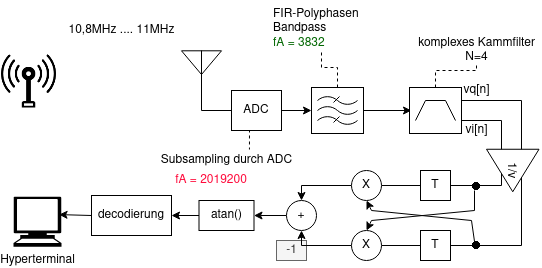
\includegraphics[width=\textwidth]{images/signalfluss.png}
  \begin{columns}
    \begin{column}{0.5\textwidth}
       \begin{enumerate}
         \item Dezimationsstufe
         \item komplexes Kammfilter
       \end{enumerate}
    \end{column}
    \begin{column}{0.5\textwidth}
        \begin{center}
         \begin{enumerate}
          \item FM-Verzögerungsdemodulator
          \item Dekodierer
         \end{enumerate}
         \end{center}
    \end{column}
  \end{columns}
}

\section{Bestimmung der Abtastfrequenzen}
\frame{
  \frametitle{Bandbreitenbestimmung}
  \begin{columns}
    \begin{column}{0.3\textwidth}
      Die Bandbreite $B = 704Hz $ wurde ausgehend von $fT$ bestimmt, 
      dass Nutzsignal fällt in den Bereich in dem $99\%$ der Signalenergie liegen.
    \end{column}
    \begin{column}{0.7\textwidth}
      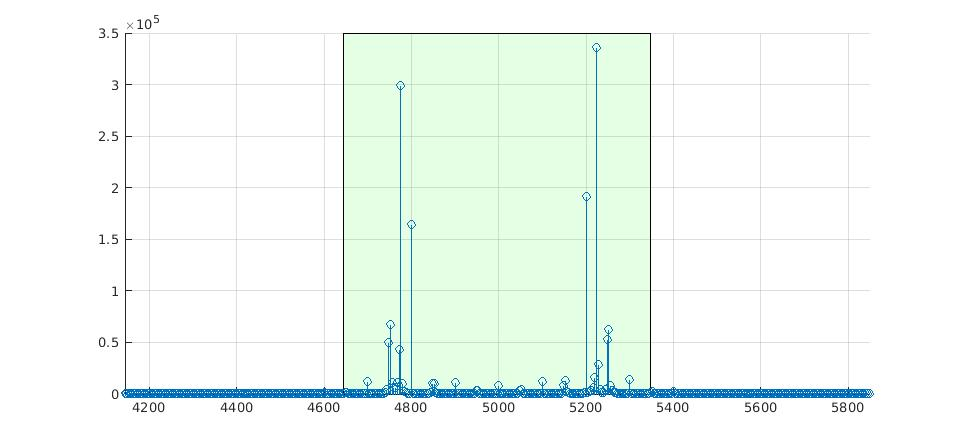
\includegraphics[width=\textwidth, height=0.7\textheight]{images/bandbreiten.jpg}
    \end{column}
  \end{columns}
}
\begin{frame}
.
  \frametitle{Bestimmung der Abtastfrequenzen}
  \begin{columns}
    \begin{column}{0.5\textwidth}
      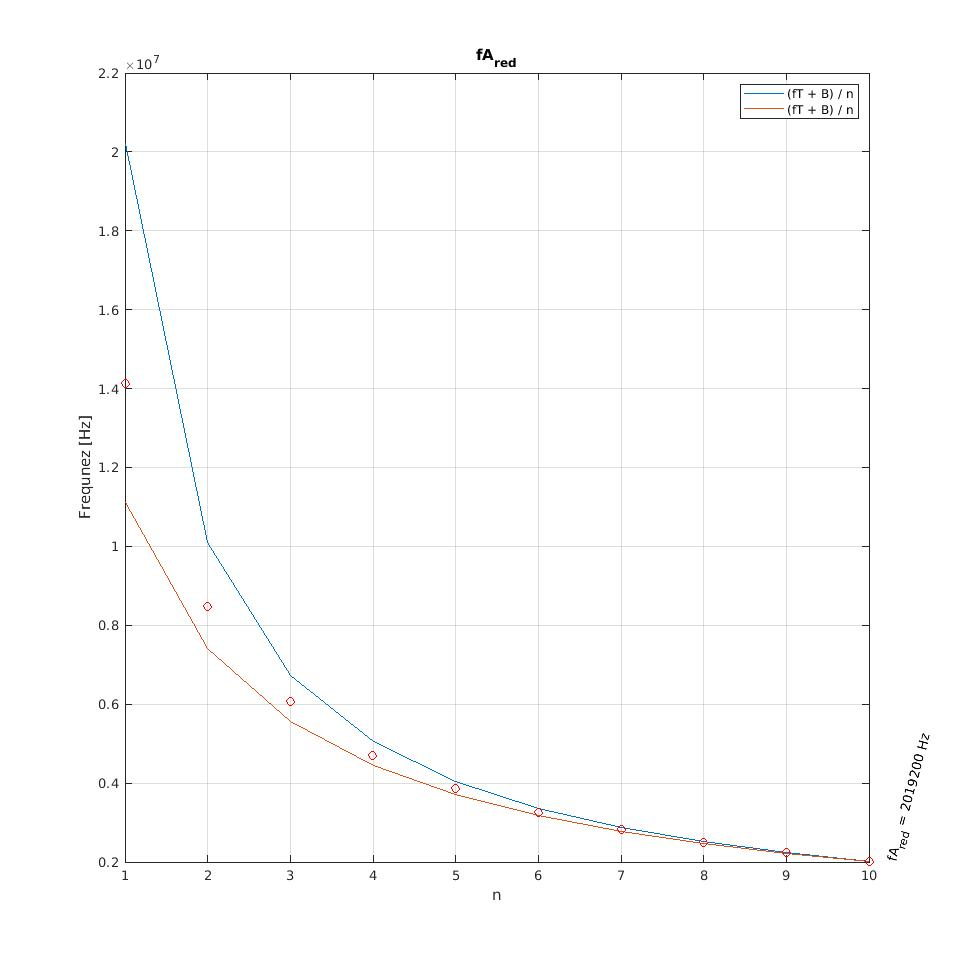
\includegraphics[width=\textwidth, height=0.7\textheight]{images/fAred.jpg}
    \end{column}
    \begin{column}{0.5\textwidth}
      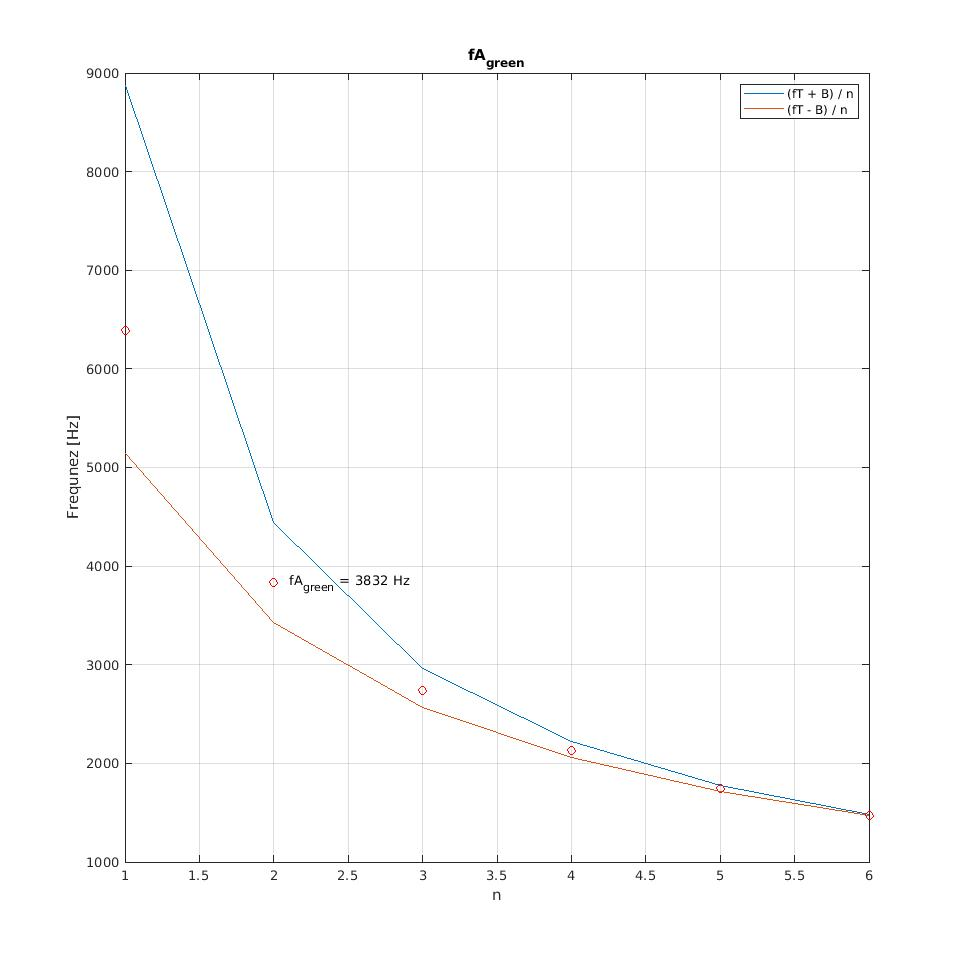
\includegraphics[width=\textwidth, height=0.7\textheight]{images/fAgreen.jpg}
    \end{column}
  \end{columns}
\end{frame}

\section{Dezimationsstufe}
\frame{
  \frametitle{Dezimationsstufe}
  \begin{columns}
    \begin{column}{0.5\textwidth}
      Vorgehen
      \begin{enumerate}
        \item In MATLAB Bandpass als FIR-Filter ausgelegt
        \item Dezimationsfaktor bestimmt: $\frac{fA_{red}}{fA_{green}} \approx 527$
        \item Polyphasen als \textit{const short} exportieren
        \item ANSI-C Implementierung
      \end{enumerate}
    \end{column}
    \begin{column}{0.5\textwidth}
        \begin{itemize}
          \item performanter ANSI-C Code durch Pointer
          \item Vermeidung von Schleifen
        \end{itemize}
    \end{column}
  \end{columns}
}

\frame{
  \frametitle{Dezimationsstufe in MATLAB}
  \begin{columns}
    \begin{column}{0.5\textwidth}
      Iteratives Vorgehen bis die Koeffizientenanzahl 
      annehmbar ist.
      \begin{itemize}
        \item Festlegung der Grenzfrequenzen $f_u = 3800Hz$ und $f_o = 4500Hz$
        \item Abschätzen der Start-/Stopfrequenzen $f_{start/stop} = f_{u/o} \pm 1500Hz$
      \end{itemize}
    \end{column}
    \begin{column}{0.5\textwidth}
      Bei dem hier gezeigten Amplitudengang werden 2056 Koeffizienten benötigt.
      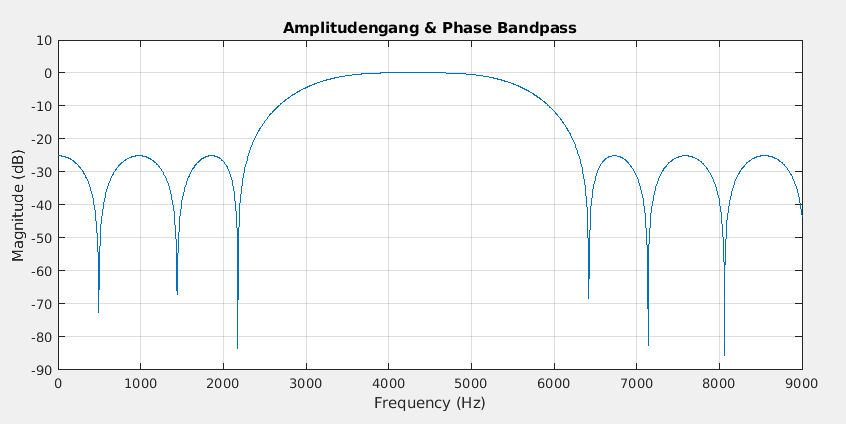
\includegraphics[width=\textwidth]{images/FIR_BP.png}
    \end{column}
  \end{columns}
}

\begin{frame}[fragile]
  \frametitle{Dezimationsstufe in ANSI-C}
  \begin{columns}
    \begin{column}{0.7\textwidth}
      \begin{itemize}
        \item Die Filterpolyphasen werden in einem Array gespeichert.
        \item Die einzelnen Polyphasen, werden nach und nach dem FIR übergeben, gefiltert und dezimiert. 
        \item Durch das Dezimieren wird das Signal ein weiteres mal unterabgetastet ($fA_{green} = 3832Hz$).
        \item Das eigentliche Nutzsignal wird in das Basisband gemischt.
      \end{itemize}
    \end{column}
    \begin{column}{0.7\textwidth}

    \end{column}
  \end{columns}
  
\end{frame}

\section{Hilbert Transformator}

\frame{
  \frametitle{Hilbert Transformator}
  \begin{columns}
    \begin{column}{0.5\textwidth}
      \begin{itemize}
        \item $x(t)_+ = x(t) \cdot \mathcal{H}\{x(t)\} $
        \item $Y(f) = -j sign(f) \cdot X(f)$
        \item als erster Ansatz zum Wandel in ein komplexes Signal
        \item nicht tauglich aufgrund der Symmetrie des Sinus
      \end{itemize}
    \end{column}
    \begin{column}{0.5\textwidth}
      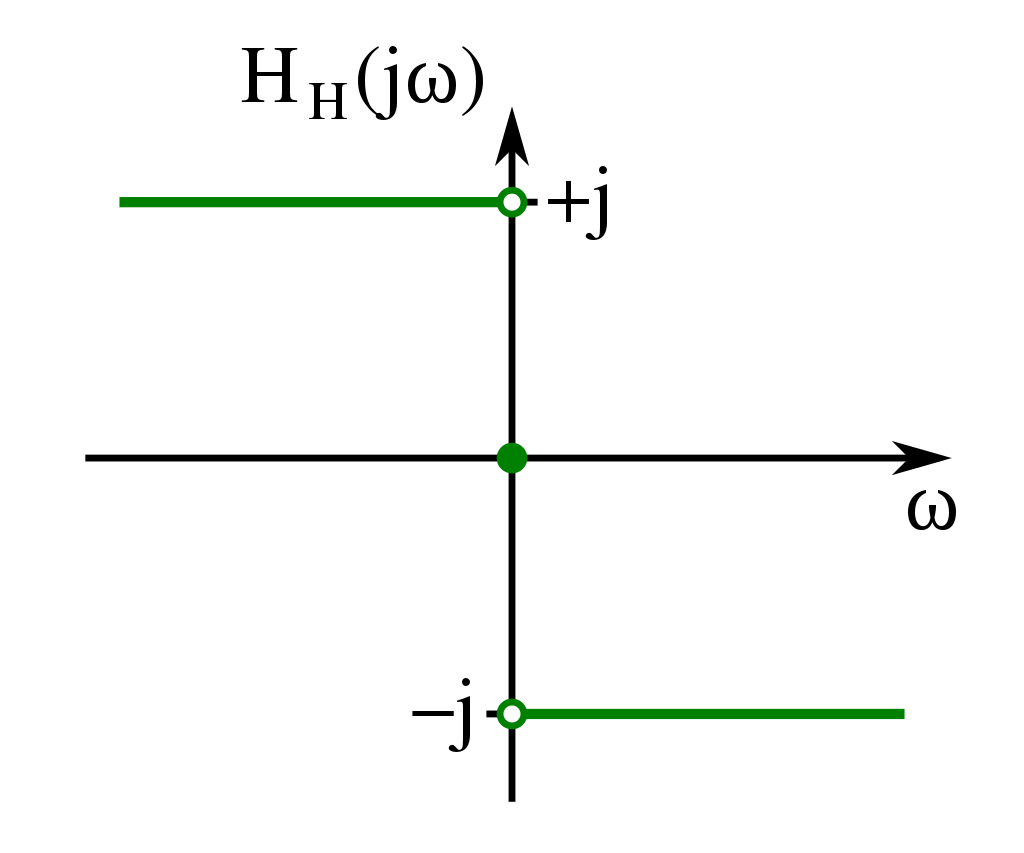
\includegraphics[height=0.4\textheight]{images/hilberto.png}
      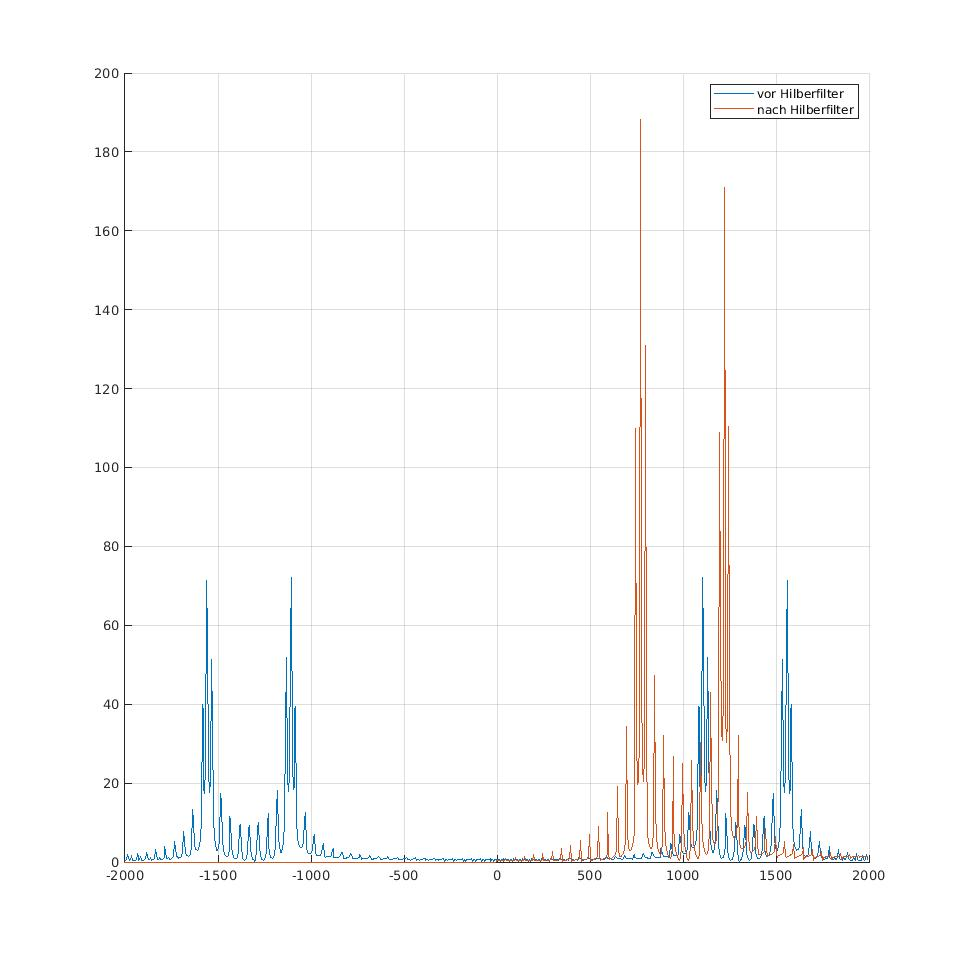
\includegraphics[height=0.6\textheight]{images/hilber_vgl.jpg}
    \end{column}
  \end{columns}
}

\section{FM-Verzögerungsdemodulator}

\begin{frame}
	\frametitle{Verzögerungsdemodulator}
	\begin{figure}
		\centering
		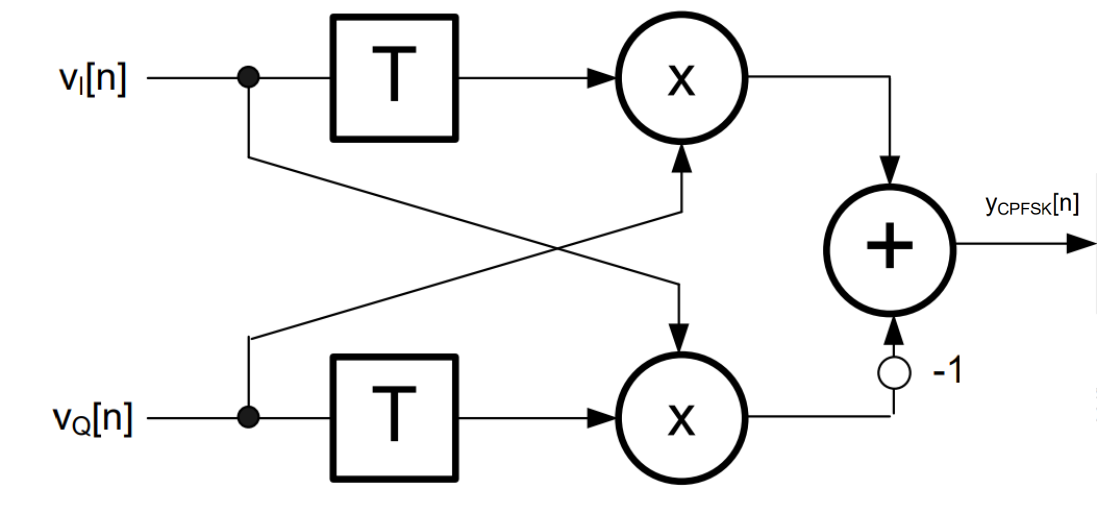
\includegraphics[height=0.4\textheight]{images/fm_demod_no_asin}
		\label{fig:fmdemodnoasin}
	\end{figure}

	\begin{columns}
		\begin{column}{0.5\textwidth}
			\begin{figure}
				\centering
				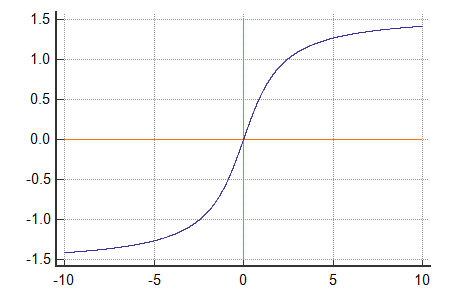
\includegraphics[width=0.8\linewidth]{images/asin}
				\label{fig:asin}
			\end{figure}
			
		\end{column}
		\begin{column}{0.5\textwidth}
			\begin{figure}
				\centering
				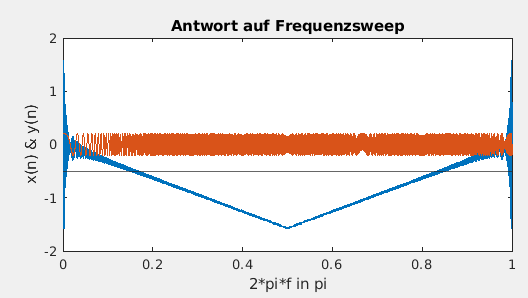
\includegraphics[width=0.8\linewidth]{images/fm_demod_sweep}
				\label{fig:fmdemodsweep}
			\end{figure}
			
		\end{column}
	\end{columns}
\end{frame}

\frame{
	\frametitle{Verzögerungsdemodulator nach Hilbert}
  \begin{columns}
    \begin{column}{0.4\textwidth}
      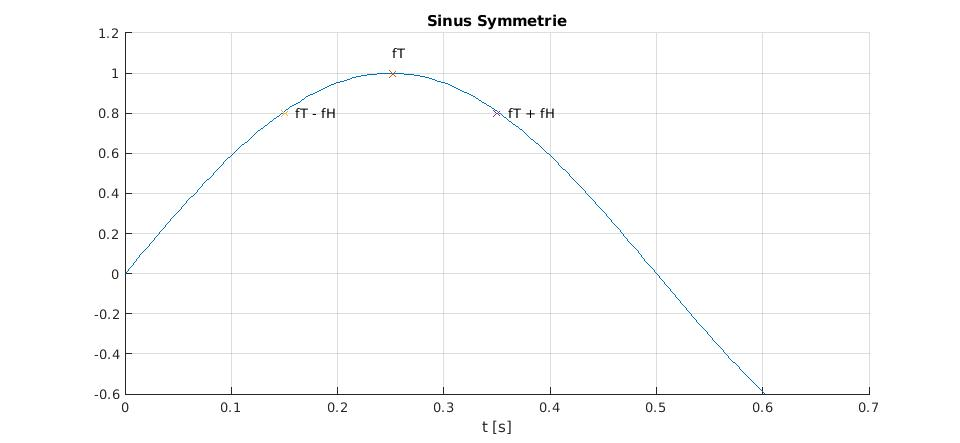
\includegraphics[height=0.3\textheight]{images/sin.jpg}
   \end{column}    
   \begin{column}{0.6\textwidth}
     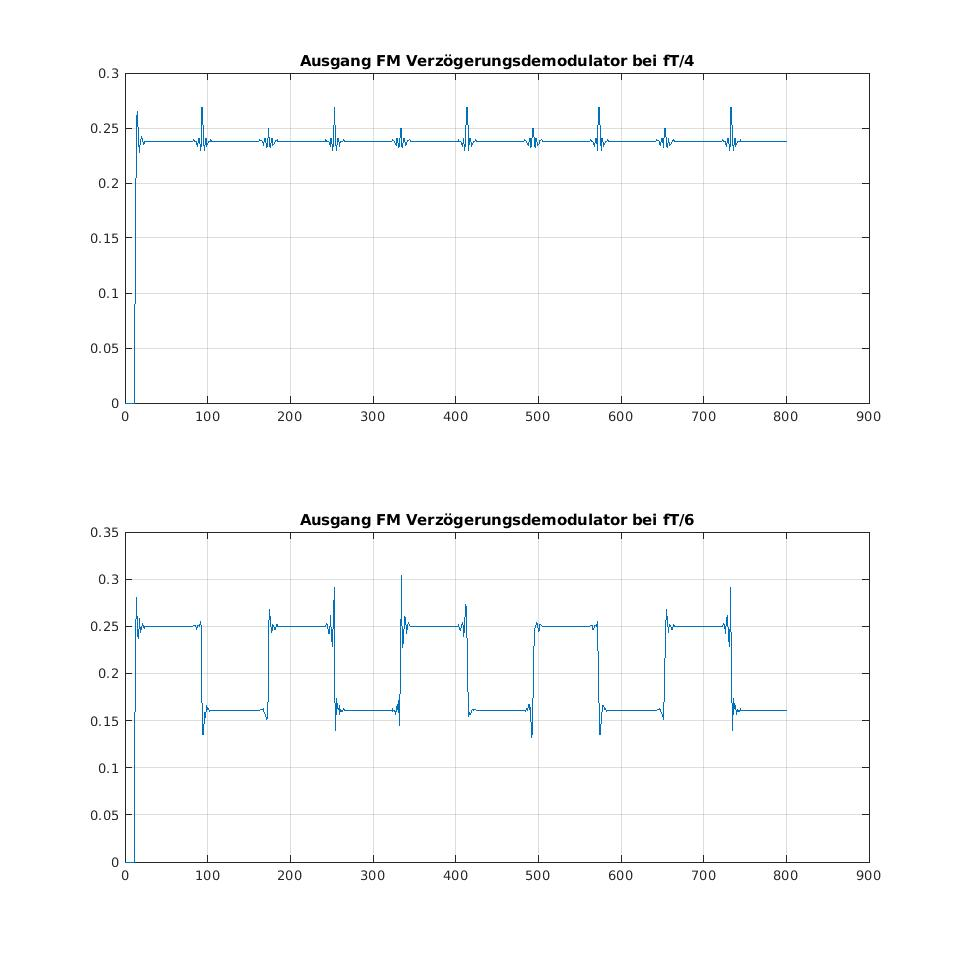
\includegraphics[height=0.6\textheight]{images/rect_demod.jpg}
     \begin{itemize}
       \item Bei ungeeigneter Trägerfrequenz, ist das Signal nicht mehr demodulierbar.
     \end{itemize}
   \end{column}
  \end{columns}
}



\section{Komplexes Kammfilter}
\frame{
	\frametitle{Komplexes Kammfilter}
	\begin{columns}
		\begin{column}{0.5\textwidth}
			Auslegung
			\begin{itemize}
				\item Festlegen des Abstandes von Maximum zu Nullstelle
				\item Anzahl der Verzögerer bestimmen
				\item Maximum auf mit DFT Verschiebungstheorem $\omega_{mark}$ verschieben
			\end{itemize}
		\end{column}
		\begin{column}{0.5\textwidth}
			\begin{itemize}
				\item $H(e^{j\omega}) = 1 + e^{j\omega u}$ mit $H(e^{j\omega})\arrowvert_{\omega = \frac{\varDelta f}{fA} \cdot 2\pi} = 0$
				\item $ u = \lfloor \frac{\pi}{2 \pi \frac{\varDelta f}{fA}} \rfloor = 4$
				\item $X(n+l) \Longleftrightarrow x(n) \cdot W^{kl}_N$
				\item $ W^{kl}_N = e^{\cfrac{-j2\pi kl}{N}}$
				\item $ h(k) \cdot e^{-j\omega_{mark}\cdot k}$
				\item $h(k) = \{ 1, 0, 0, 0, 0.175 - i0.985\}$
			\end{itemize}
		\end{column}
	\end{columns}
}

\begin{frame}
	\frametitle{Komplexes Kammfilter}
	\begin{columns}
		\begin{column}{0.3\textwidth}
			
			\begin{itemize}
				\item jeweils eine Frequenz wird gedämpft
				\item Nullstellen sind verschoben
				\item Es entsteht ein komplexes Signal
			\end{itemize}
		\end{column}
		\begin{column}{0.7\textwidth}
			Amplitudengang
			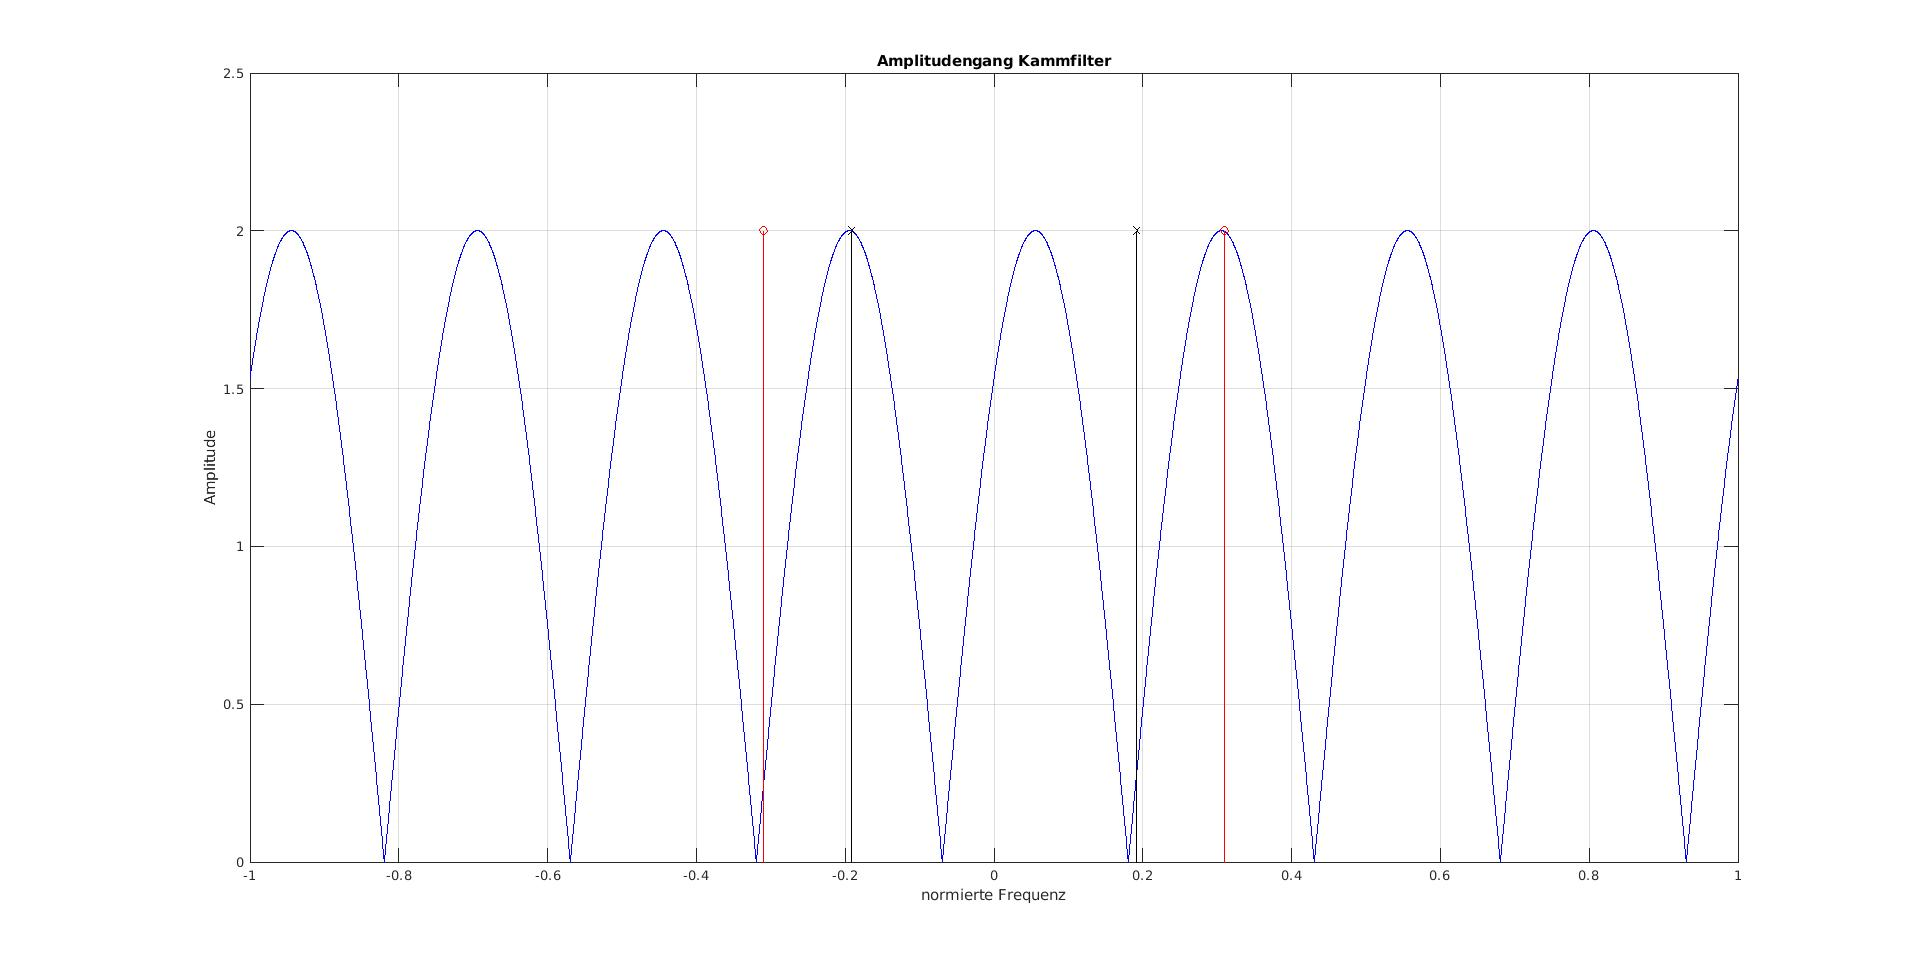
\includegraphics[width=\textwidth]{images/comb.png}
		\end{column}
	\end{columns} 
	  -\\
	Verzögerungsdemodulator ist für eine Frequenz invertiert.
	$sin(-\omega_{mark}) = -sin(\omega_{mark}) = -sin(\omega_{space}) \Longleftrightarrow sin(\omega_{space})$
\end{frame}

\frame{
	\frametitle{Ergebnis}
  Ausgänge und Spektren der Filterstufen 
  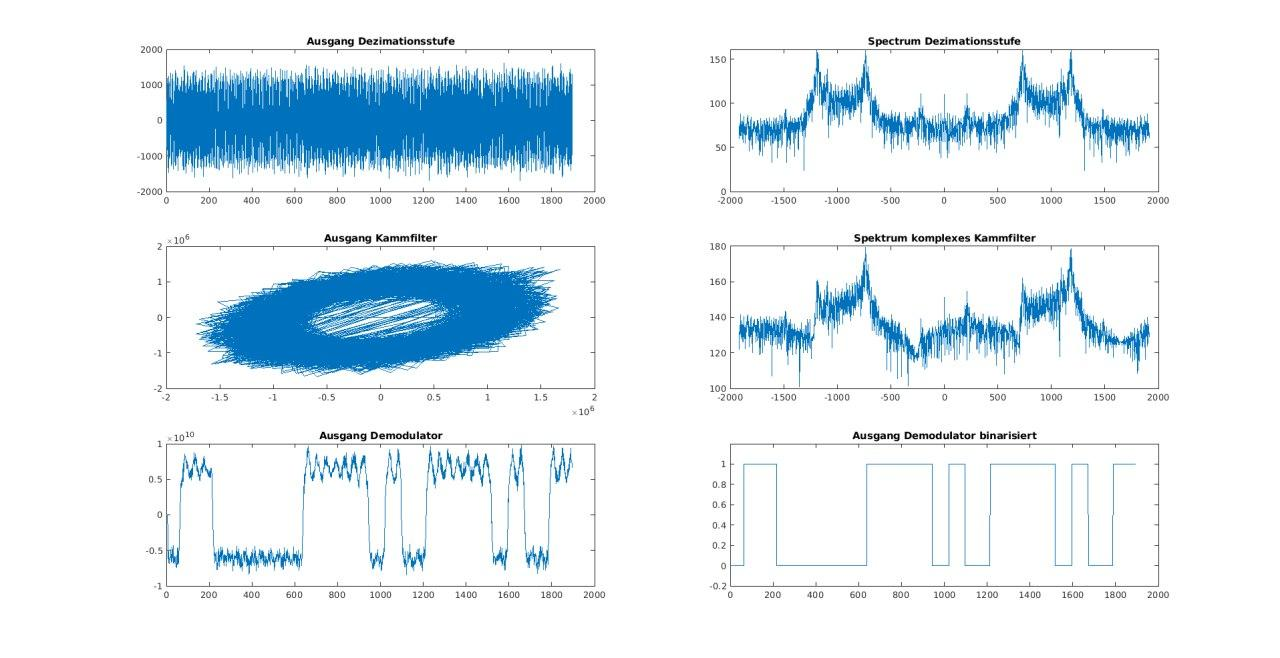
\includegraphics[width=1\textwidth]{images/result.jpg}
	\begin{columns}
		\begin{column}{0.5\textwidth}
			
			\begin{itemize}
				\item Ergebnisse entsprachen in der C-Simulation den Erwartungen.

			\end{itemize}
		\end{column}
		\begin{column}{0.5\textwidth}
			\begin{itemize}

				\item Signal wurde korrekt demoduliert.
			\end{itemize}
		\end{column}
	\end{columns}
}

\section{Dekodierer}
\frame{
  \frametitle{Dekodierer}
  \begin{columns}
    \begin{column}{0.5\textwidth}
      \begin{itemize}
        \item demoduliertes Rechtecksignal wird nochmal untertastet um Faktor 38.31
        \item dekodierte Symbole als Index für Lookuptable
        \end{itemize}
      \end{column}
  \end{columns}
}

\frame{
	\frametitle{Dekodierer - ANSI C}
	
	\begin{figure}
		\centering
		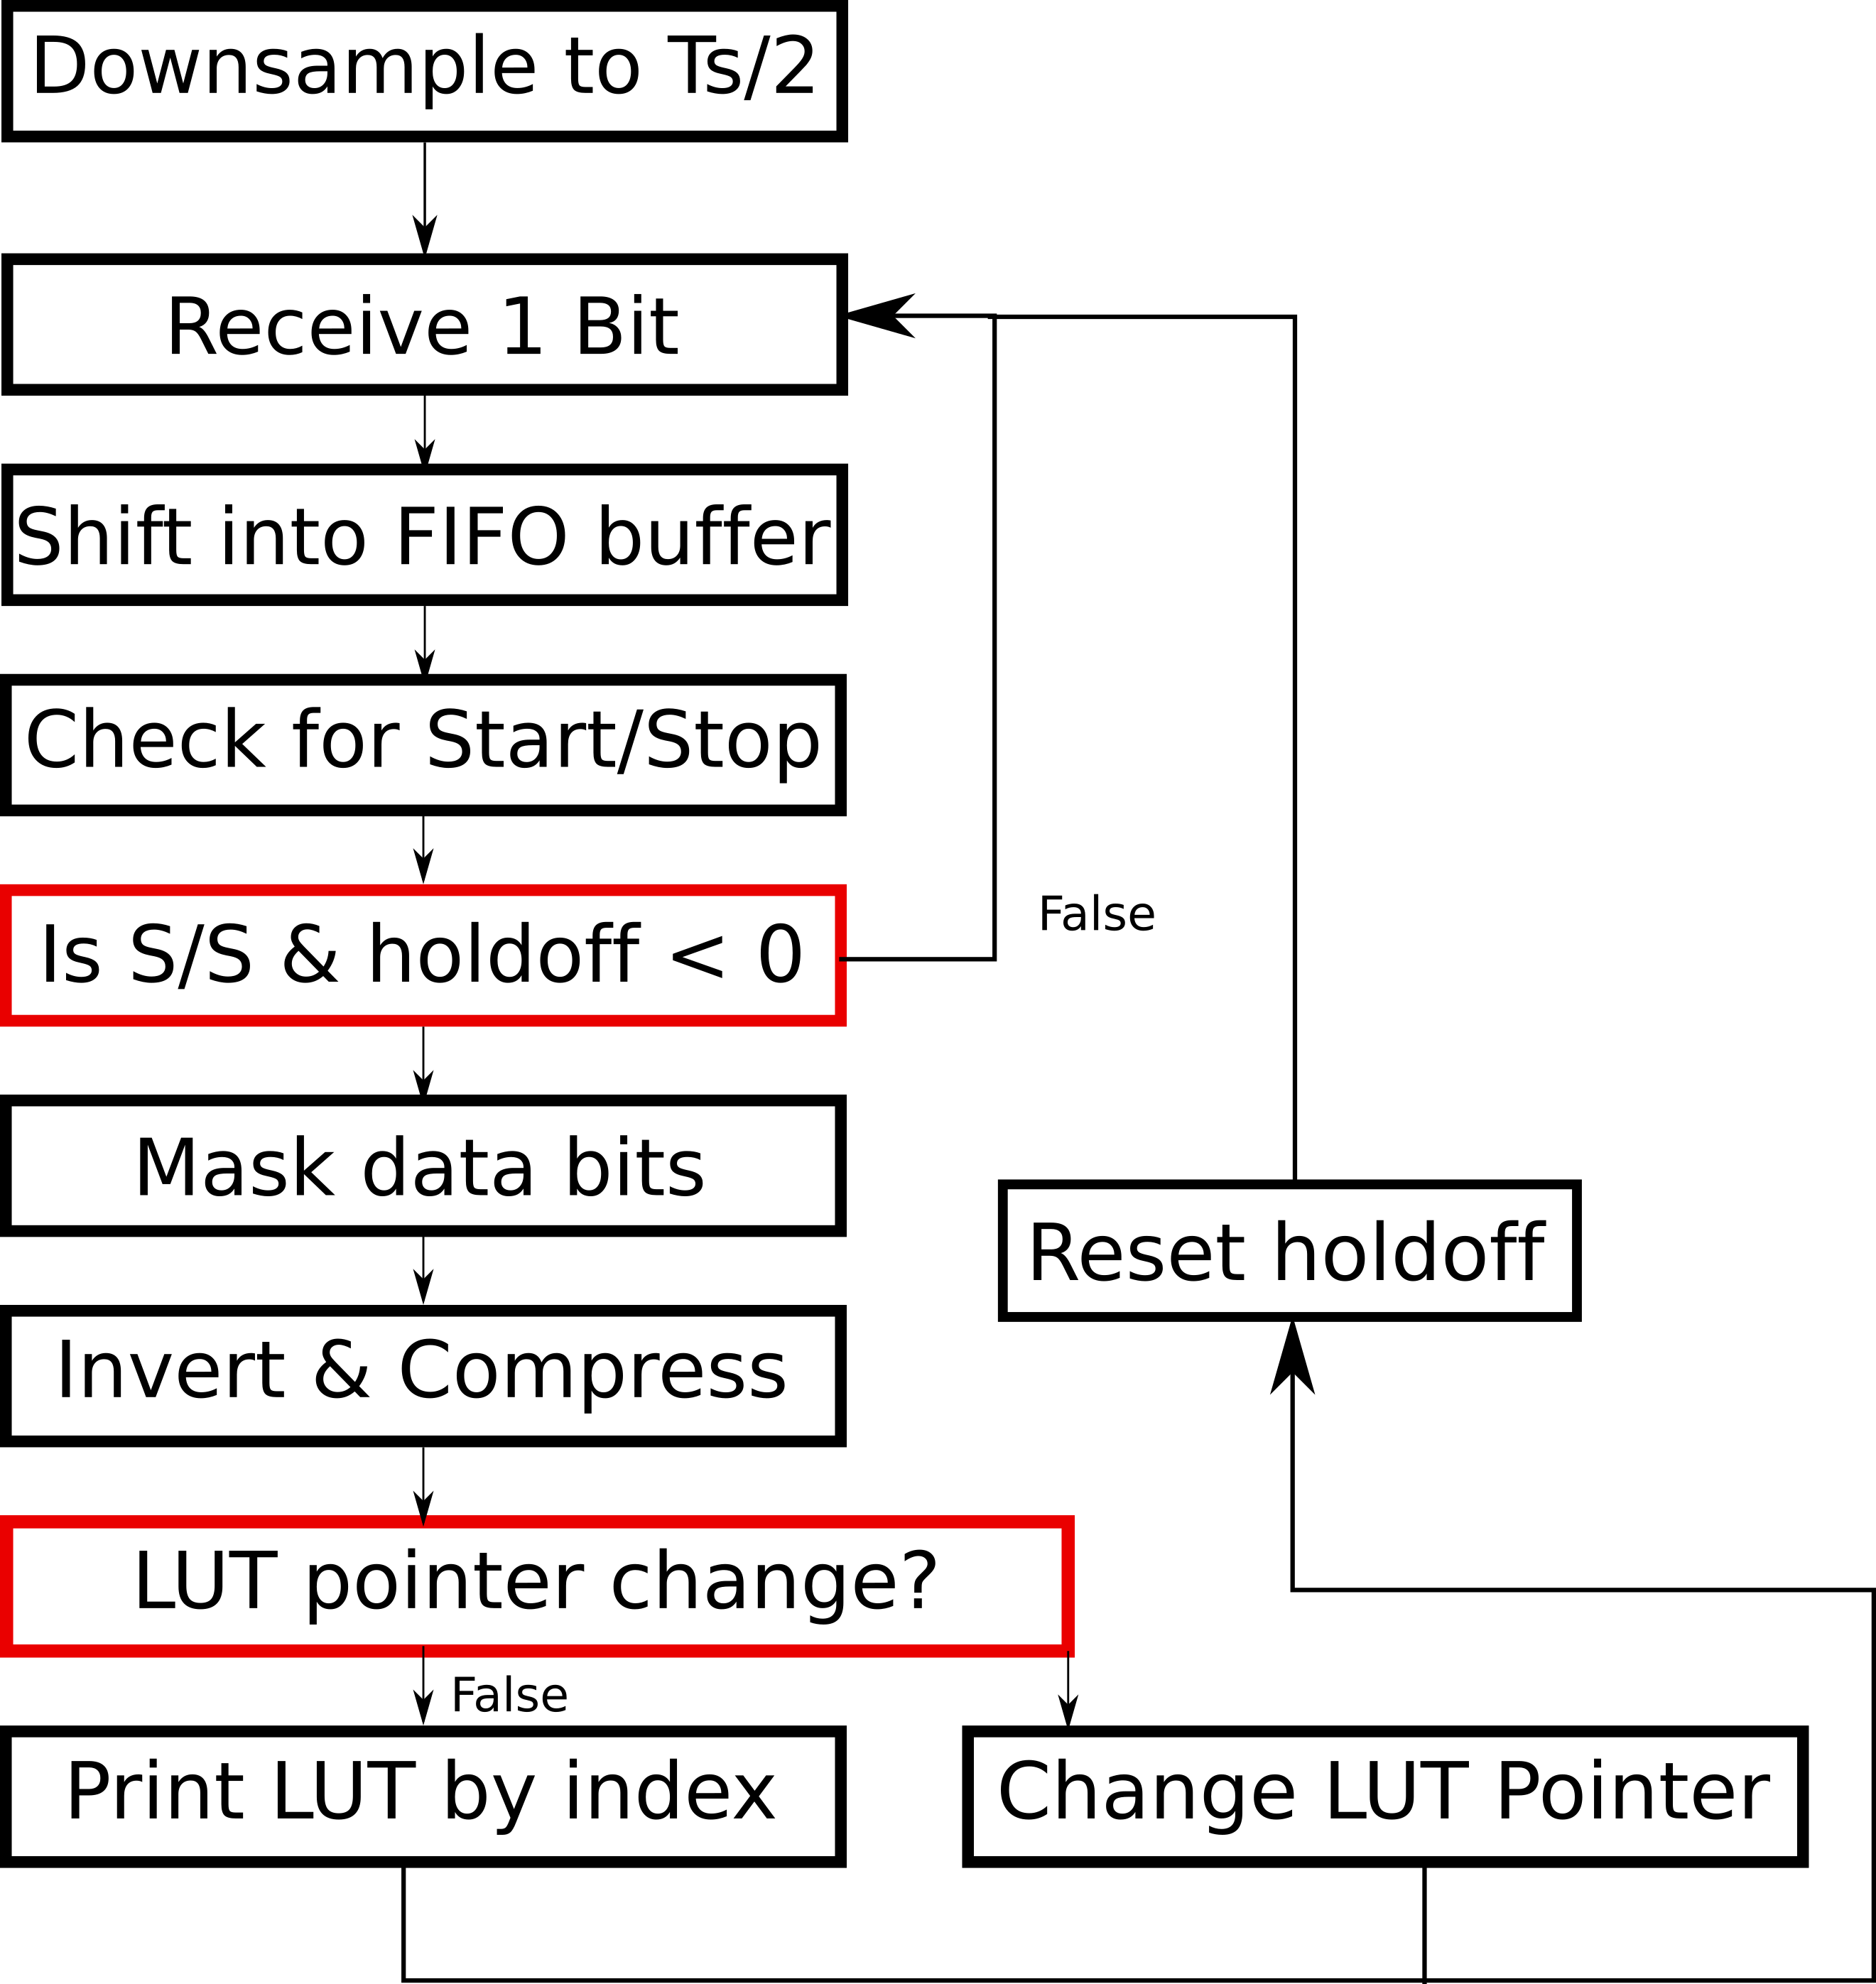
\includegraphics[width=0.6\linewidth]{images/rect833}
		\label{fig:rect833}
	\end{figure}
	
}


\begin{frame}[fragile]
	\frametitle{Implementierung Dekodierer}
	
	\begin{lstlisting}[basicstyle=\tiny,style=CStyle]			
buffer = buffer << 1; // Shift FIFO left
buffer = buffer | bit; // Enter bit
startstop = buffer & 0x001F; // Mask size of start/stop

if (startstop_holdoff > 0) // Underflow protection
	startstop_holdoff -= 1;

if (startstop == STOP_SEQUENCE && startstop_holdoff == 0) {
	startstop_holdoff = 11;
	index_pre = (buffer >> 5) & 0x03FF; 
	real_index =  (((index_pre >> 0) & 0x0001) << 4) 
		   		   	| (((index_pre >> 2) & 0x0001) << 3) 
							| (((index_pre >> 4) & 0x0001) << 2) 
							| (((index_pre >> 6) & 0x0001) << 1) 
							| (((index_pre >> 8) & 0x0001) << 0);

	if (real_index == SWITCH_TO_CHAR) {
		current_lut = lookup_char;
	} else if (real_index == SWITCH_TO_NUM) {
		current_lut = lookup_num;
	} else {
		printf(" >> %c <<\n",current_lut[real_index-1]); 
	}
}

\end{lstlisting}
\end{frame}

\section{Fazit}
\frame{
  \frametitle{Fazit}
  \begin{columns}
    \begin{column}{0.6\textwidth}
      
      \begin{itemize}
        \item interessantes und herausforderndes Projekt
        \item weitere Optionen: Optimalfilter zu SNR Verbesserung, Demodulation mit Komperator
        \item Umstände mit Corona sehr schade
       
      \end{itemize}
    \end{column}
    \begin{column}{0.4\textwidth}
      Dekodiertes Testsignal
      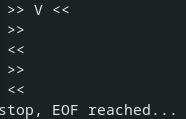
\includegraphics[width=0.6\textwidth]{images/term.png}
      \end{column}
  \end{columns}
}

% that's all, folks
\end{document}
